\chapter{Computer Networks and the Internet (1-78)}


\lecture{1}{19 Feb}{1-5}

\section{What Is the Internet}

\begin{definition}[public internet]\label{def:public_internet_1}
    Specific computer network, a system that connects two or more computing devices to transmit and share information.
\end{definition}

\begin{definition}[computing device]\label{def:computing_device_1}
    A functional unit that can perform substantial computations, including numerous arithmetic operations and logic operations without human intervention. A computing device can consist of a standalone unit or several interconnected units. It can also be a device that provides a specific set of functions, such as a phone or a personal organizer, or more general functions such as a laptop or desktop computer. 
\end{definition}

\begin{definition*}
    The internet can be defined in two ways.
\begin{definition}[nuts and bolts]\label{def:internet_def_1}
    Basic hardware and software components that make up the Internet.
  \end{definition}
  \begin{definition}[networking infrastructure]\label{def:internet_def_2}
     Networking infrastructure that provides services to distributed applications. 
     The hardware and software that enable network connectivity and communication between users, devices, apps, the internet, and more.
  \end{definition}
\end{definition*}
\newpage

    \subsection{A nuts-and-Bolts Description}
        \begin{definition}[Computer network]\label{def:computer_network_1}
            Interconnects billions of computing devices throughout the world\footnote{Since even devices different than computers are hooked to the Internet this term can be considered outdated}.    
        \end{definition}

\begin{note}[what connects end systems]\label{note:end_systems_1}
        End systems are connected by communication links and packet switches.
\end{note}

\begin{note}[transmission rate]\label{note:transmission_rate_1}
    The transmission rate of a link is measured in bits/second
\end{note}

\vspace{24pt}

\begin{figure}[h!]
    \centering
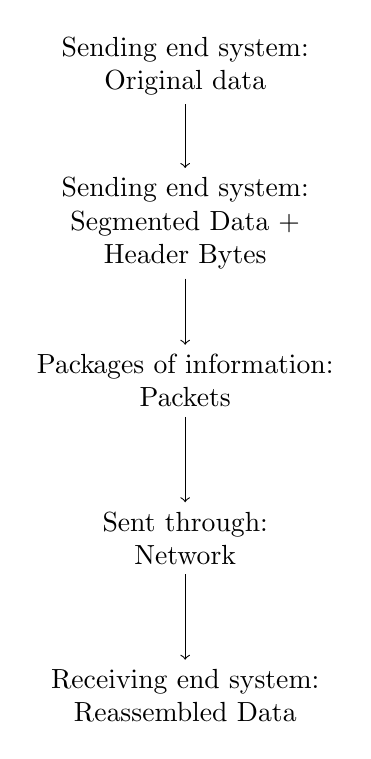
\begin{tikzpicture}[node distance=2cm, auto]

  % Nodes
  \node (data) [align=center] {Sending end system:\\ Original data};
  \node (segment) [below of=data, align=center] {Sending end system:\\ Segmented Data +\\Header Bytes};
  \node (packets) [below of=segment, align=center] {Packages of information:\\ Packets};
  \node (network) [below of=packets, align=center] {Sent through:\\ Network};
  \node (reassembled) [below of=network, align=center] {Receiving end system:\\ Reassembled Data};

  % Arrows
  \draw[->] (data) -- (segment);
  \draw[->] (segment) -- (packets);
  \draw[->] (packets) -- (network);
  \draw[->] (network) -- (reassembled);

\end{tikzpicture}
\caption{Data transmission process in a computer network}\label{fig:data_transmission_1}
\end{figure}


\vspace{24pt}

\begin{definition*}\label{def:packet_switches_1}
    Two main types of packet switches. They forward packets to their ultimate destination
        \begin{definition}[Routers]\label{def:routers_1}
           Used in network core 
        \end{definition}
        \begin{definition}[Link-layer switches]\label{def:link_layer_switches_1}
            used in access networks
        \end{definition}
\end{definition*}

\begin{definition}[route or path]\label{def:route_path_1}
    The path a packet takes from sender to receiver through communication links and switches.    
\end{definition}

\newpage

\begin{note}[end systems]\label{note:end_systems_2}
    End systems access the Internet using Internet Service Providers 
\end{note}


\begin{definition}[isp]\label{def:isp_1}
    A network of packet switches and communication links \ref{def:routers_1} \& \ref{def:link_layer_switches_1}. 
    
    They provide network access to end systems, including residential broadband access such as cable modem, local area network access and mobile wireless access. 

    They also provide Internet access to content providers, connecting different servers. 

    There are lower and upper tier of ISP, they are all managed independently and run the IP protocol, conforming to naming and address conventions.
\end{definition}

\begin{definition*}
    End systems, packet switches and other pieces of the internet run various protocols. TCP and IP are the two main one
    \begin{definition}[Transmission Control Protocol]\label{def:tcp_1}
         Enables application programs and computing devices to exchange messages over a network. It is designed to send packets across the internet and ensure the successful delivery of data and messages over networks.

         It organizes data so that it can be transmitted between a server and a client. It guarantees the integrity of the data being communicated over a network. Before it transmits data, TCP establishes a connection between a source and its destination, which it ensures remains live until communication begins. It then breaks large amounts of data into smaller packets, while ensuring data integrity is in place throughout the process.
    \end{definition}
    \begin{definition}[Internet Protocol]\label{def:IP_1}
        Specify the format of the packets
    \end{definition}

    \begin{note}[differences]\label{note:ip_vs_tcp_1}
        IP obtains and defines the address—the IP address—of the application or device the data must be sent to. TCP is then responsible for transporting and routing data through the network architecture and ensuring it gets delivered to the destination application or device that IP has defined.
    \end{note}
\end{definition*}

\begin{note}[IETF]
    Internet standards developed by the Internet Engineering Task Force. 

    Their standard documents are called \textbf{requests for comments},
    
\end{note}






\newpage


\lecture{2}{21 Feb}{5-21}


